\hypertarget{aineisto-ja-menetelmuxe4t}{%
\chapter{Aineisto ja menetelmät}\label{aineisto-ja-menetelmuxe4t}}

\hypertarget{section}{%
\section{\texorpdfstring{\gls{ddd}}{}}\label{section}}

Yleinen ongelma tietokoneohjelmistoja tehtäessä on, että ohjelmoijat
tuntevat ohjelmiston erikoisalan heikosti. Esimerkiksi
kiinteistötekniikkaa, kirjastokortistoa tai tämän työn tapauksessa
terapiaklinikan toimintaa hoitavan ohjelmiston kehittäjä joutuu
käsittelemään monimutkaisia, sovellusalaan sidottuja ongelmia.
Ohjelmiston tulisi ratkaista ongelmat oikein, ja toimia virheettömästi
kun sitä käytetään.

Eric Evans esittää kirjassaan Domain Driven Design laajan työkalupakin
keinoja, joilla tämän ongelman voi pyrkiä ylittämään. Evansin mielestä
jokaisen monimutkaisemman ohjelmiston sisässä on \gls{domainmodel}
(Domain model), eli malli siitä, miten kyseinen ohjelmisto ratkaisee
sovellusalan ongelmat.

\Gls{crunching} (Knowledge crunching) on keskeinen väline
sovellusaluemallin rakentamiseen. Evans kuvaa prosessin, jossa
kehittäjät luonnostelevat yhdessä sovellusalueen asiantuntijoiden kanssa
\gls{domainmodel}in. Malli kytketään tiiviisti yhteen ohjelmakoodin
kanssa vuorottelemalla suunnittelun ja ohjelmistokehityksen välillä.
\cite[s. 13]{evans:ddd}

Tavoitteena on, että ohjelmistokehittäjien ja alan asiantuntijoiden
välille rakentuu \gls{ubilang}, jonka avulla kaikkien on mahdollista
yhteisesti keskustella ohjelmiston toiminnasta ja kehitystarpeista.
Tämän kielen käsitteet elävät ohjelmakoodissa, ja muodostavat koodin
ytimessä sijaitsevan \gls{domainlayer}

\hypertarget{n-rakennuspalikat}{%
\subsection{\texorpdfstring{\gls{ddd}n
rakennuspalikat}{n rakennuspalikat}}\label{n-rakennuspalikat}}

Evansin lähtökohta on, että \gls{domainmodel} ilmaistaan nimenomaan
ohjelmakoodin kautta. Koodi on kuitenkin lopulta se dokumentti, joka
määrittää ohjelman toiminnan.

Evans tarjoaa kirjassaan joukon käteviä työkaluja, joiden avulla
\glsentryname{domainmodel} on mahdollista toteuttaa teknisesti.

\Gls{entity} edustaa käytännössä kaikkea, jolla on identiteetti.
Esimerkiksi kahdella ihmisellä voi olla sama nimi, mutta he ovat silti
identiteetiltään eri henkilöitä. \gls{entity} voi myös muuttaa muotoaan,
esimerkiksi ihminen kasvaa aikuiseksi ja vaikkapa vaihtaa sukunimensä.
Identiteetti säilyy silti. Todella suuri osa
\glsentryname{domainmodel}{sta} koostuu juuri
\glsentryname{entity}{ista}.

Laskutusta käsittelevässä ohjelmassa esimerkiksi laskuilla on
identiteetti. Kahdella laskulla voi olla sisällytettynä samat tuotteet
ja maksajakin voi olla sama, mutta silti laskut ovat omia erillisiä
kokonaisuuksiaan.

Tärkeä osa mallia ovat myös kulkusuunnat \glsentryname{entity}{iden}
välillä. Nämä vaikuttavat paitsi ohjelmiston tekniseen
monimutkaisuuteen, myös siihen, minkälaisia asioita mallilla on
mahdollista ilmaista.

Esimerkiksi lasku voi koostua joukosta laskurivejä. Ohjelman toteutus ja
käyttötavat muuttuvat hyvin paljon, jos kulkusuuntaa muutetaan.

\begin{itemize}
\tightlist
\item
  Tapaus A: lasku tietää, mitkä laskurivit siihen kuuluvat, mutta
  yksittäinen laskurivi ei tiedä, miltä laskulta on peräisin.
\item
  Tapaus B: laskurivi osaa kertoa, mille laskulle se kuuluu, mutta lasku
  ei kykene listaamaan omia rivejään.
\end{itemize}

Kolmas vaihtoehto on mahdollistaa kulkeminen molempiin suuntiin näiden
kahden käsitteen välillä. Tällöin ohjelman tekninen monimutkaisuus
kasvaa.

\hypertarget{refaktorointi}{%
\section{Refaktorointi}\label{refaktorointi}}

Yleistä refaktoroinnista

\begin{itemize}
\tightlist
\item
  Refactoring towards deeper insight
\item
  YAGNI-periaate
\item
  Automaattiset yksikkötestit (Clean Code vai XP -kirja? - uncle bobin
  ``Three laws of TDD'' -blogi)
\end{itemize}

\hypertarget{graphql}{%
\section{GraphQL}\label{graphql}}

Monet web-sovellukset perustuvat REST-rajapintoihin. REST on
arkkitehtuurityyli, jossa palvelin esittää asiakasohjelmalle joukon
resursseja, joita asiakasohjelma voi pyytää ja muunnella tilattomia
pyyntöjä käyttäen.\cite{fielding2000architectural}

REST-tyyli on vakiintunut web-sovellusten toteuttamisteknologiaksi,
mutta siihen liittyy myös eräitä ongelmia. Mikäli REST-tyyppisestä
rajapinnasta halutaan hakea usean eri resurssin verkko, joudutaan
tekemään erillinen pyyntö jokaista resurssia kohti. Toisissa tapauksissa
taas halutaan vain osa resurssin esittämästä tiedosta, mutta joudutaan
silti hakemaan koko
resurssi.\cite{betterRESTPrisma}\cite{WhyUseGraphQLApollo}

GraphQL on Facebookin kehittämä kyselykieli, joka on tarkoitettu
rajapintojen toteuttamiseen. Sen alkuperäinen suunnitteluperiaate oli
tarjota web-asiakasohjelmien kehittäjille aiempaa laajempi vapaus
rajapintapyyntöjen laatimiseen. \cite{graphql:spec}

GraphQL on vielä suhteellisen uusi teknologia, eikä siitä löydy kovin
paljoa materiaalia. Keskeinen tiedonlähde ovat Facebookin ja
GraphQL-säätiön julkaisemat verkkomateriaalit, sekä Apollo-yrityksen
GraphQL-teknologiaa käsittelevä materiaali.

GraphQL koostuu kahdesta osasta: kyselykielestä sekä
tyyppijärjestelmästä. Kyselykielellä muotoillaan pyyntö, johon
GraphQL-palvelun tulee vastata.

GraphQL ei ole varsinainen rajapinta, sillä rajapinnan
toteuttamisteknologia on määrittelyn ulkopuolella. Useimmiten
GraphQL-palvelut on toteutettu HTTP-teknologian päälle, mutta muitakin,
kuten WebSocketia, voi käytttää. GraphQL ei myöskään määrittele, miten
kyselyn vastaus tulee muodostaa, tai milllä ohjelmointikielellä
järjestelmä tulee toteuttaa.

Osa konventioista on JavaScript-konventioita. Esimerkiksi kentän- ja
muuttujien nimet on tapana kirjoittaa camelCase- ja PascalCase
-muodoissa.\cite{GraphQLSchemaBasics}

\hypertarget{miten-graphql-sovellus-toimii}{%
\subsection{Miten GraphQL-sovellus
toimii}\label{miten-graphql-sovellus-toimii}}

\begin{figure}
\centering
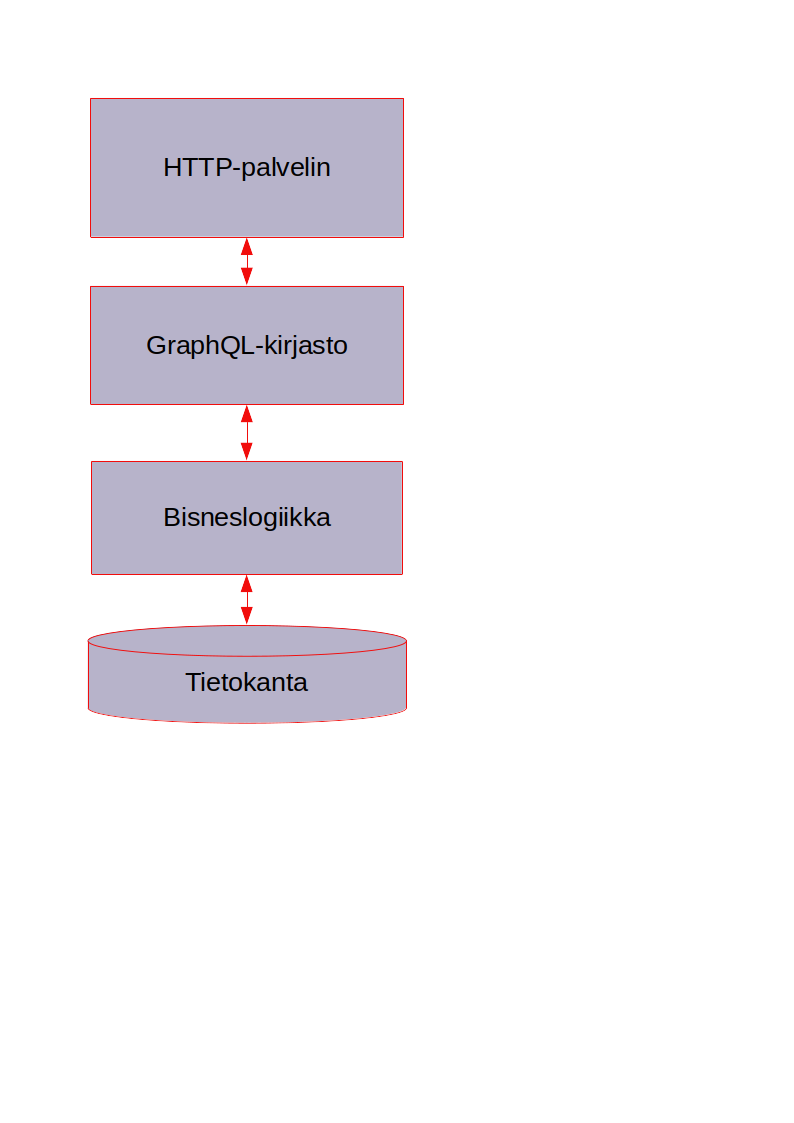
\includegraphics[width=\textwidth,height=0.5\textheight]{illustration/GraphQL-arkkitehtuuri.png}
\caption{\label{graphqlarkkitehtuuri} Esimerkkiarkkitehtuuri
GraphQL-sovellukselle}
\end{figure}

Kuvassa \ref{graphqlarkkitehtuuri} esitän yksinkertaisen
GraphQL-sovelluksen arkkitehtuurin. Arkkitehtuuri on kerroksittainen, ja
rajapinnalle esitettävä pyyntö liikkuu siinä ylhäältä alaspäin.

Ensiksi pyyntö saapuu HTTP-palvelimeen. Tämä palvelin on käytännössä
ohjelmointikielestä riippuen kirjasto, joka vastaanottaa HTTP-pyyntöjä
ja osaa käsitellä niitä. Tyypillisesti GraphQL-rajapinnassa on vain yksi
\texttt{graphql}-niminen resurssi, jolle pyynnöt esitetään.

HTTP-kerros ottaa pyynnön vastaan, ja lukee sen body-osassa olevan
merkkijonomuotoisen GraphQL-kyselyn. Tämä kysely on tehty
GraphQL-kyselykielellä. Rajapinta antaa kyselyn GraphQL-kirjastolle.

Kirjasto ottaa kyselyn vastaan, ja tarkistaa sen oikeellisuuden
GraphQL-skeemaa vasten. Mikäli kysely on muodoltaan oikeanlainen,
kirjasto ohjaa sen eteenpäin resolvereiksi kutsutuille funktioille.
Resolver-funktiot eivät ole osa kirjastoa, vaan sovelluksen kehittäjä
kirjoittaa ne. Käytännössä resolver-funktio on nk. puhdas funktio, jonka
tehtävänä on tuottaa vastaus yksittäiseen GraphQL-kyselyn kenttään.

Laskutusta käsittelevässä esimerkissä rajapinnan invoices-kenttää voisi
vastata \texttt{invoices\_resolver} -niminen funktio.

Resolver-funktioiden kerros on alin kerros, josta GraphQL-palvelu
tietää. Sen alla oleva ohjelmistologiikka on riippumaton rajapinnan
toteutustavasta. Tyypillisesti siellä voi sijaita sovelluksen
liiketoimintalogiikka, ja tietokanta.

\hypertarget{graafeista}{%
\subsection{Graafeista}\label{graafeista}}

Graafi eli verkko on tietorakenne, joka koostuu N:stä solmusta ja niitä
yhdistävistä kaarista.\cite{pozrikidis2014introduction} Graafien avulla
on mahdollista esittää monenlaisia suhdeverkkoja. Tietojenkäsittelyssä
ja ohjelmistotuotannossa yleinen olio-ohjelmoinnin tyyli esittää
ratkaistavan ongelmakentän olioiden välisinä
verkkoina.\cite{booch2008object}

GraphQL:n avulla sovellusala on mahdollista esittää verkon muodossa
määrittelemällä GraphQL-skeema. Tämän avulla rajapinta tarjoaa
asiakasohjelmalle rakenteen, joka muistuttaa
olio-ohjelmointia.\cite{thinkingInGraphsOct2021}

\begin{itemize}
\tightlist
\item
  tähän vielä vähän lisää funtsailua siitä, miten olio-ohjelmoinnin
  graafimainen ajattelu ohjaa ongelmanratkaisua, ja ehkä myös joku
  naseva pätkä Evansilta samansuuntaisesti ajattelemiseen
\end{itemize}

\hypertarget{tyyppijuxe4rjestelmuxe4}{%
\subsection{Tyyppijärjestelmä}\label{tyyppijuxe4rjestelmuxe4}}

Tietokoneet käsittelevät dataa ottamatta sen enempää kantaa sen
tyyppiin. Pohjimmiltaan data on vain bittijonoja muistissa, tai
elementtejä joukossa. Kun tällaista järjestämätöntä ja tyypittämätöntä
joukkoa ryhdytään käsittelemään, on välttämätöntä järjestää se
erilaisiin kategorioihin. Tämä tiedon luokittelu synnyttää
tyyppijärjestelmän, mutta järjestelmä ei ole formaalisti määritelty,
eikä tietokone voi niin ollen tehdä tyyppitarkistusta.

Tyypitys tarkoittaa määrättyjä rajoituksia, joiden avulla voidaan
varmistaa muuttujan oikeellisuus. Staattinen tyypitys on menetelmä,
jossa ekspressioiden tyyppi voidaan määrittää staattisen analyysin
avulla, siis jo käännösaikaisesti. Vahva tyypitys taas mahdollistaa
tyypin tarkistamisen luotettavasti ajon aikana.
\cite{Cardelli+Wegner:1985}

GraphQL-rajapinta koostuu tyypeistä, joita rajapinnalle lähetettävä
kysely käyttää. Kyselyssä määritetään pyydettävät tyypit ja niiden
kentät. Rajapinta palauttaa takaisin oliota edustavan joukon kenttiä
\gls{hakurakenne}-muodossa. \cite{graphql:spec}

GraphQL:ää käyttävät sovellukset on kuitenkin useimmiten kirjoitettu
dynaamisesti tyypitetyillä kielillä. Esimerkiksi alkuperäinen
GraphQL-referenssi-implementaatio on kirjoitettu
JavaScriptillä.\cite{graphqlRefImple2021Oct}

Samoin Python-kieli on dynaamisesti tyypitetty, ja olioiden
tunnistamisessa se käyttää duck-tyypitykseksi kutsuttua menetelmää.
Duck-tyypityksessä olion tyyppiä ei tarkasteta välttämättä edes
ajonaikaisesti, vaan oletetaan sen sisältämien jäsenten
perusteella.\cite{pythonGloss2021Oct} Jos esimerkiksi oliosta löytyvät
kentät \emph{summa} ja \emph{laskunumero}, oletetaan, että olio on
lasku.

Tässä mielessä voidaan ajatella, että GraphQL on keino tuoda
ajonaikaisia tyyppitarkistuksia myös dynaamisesti tyypitetyillä kielillä
kirjoitettuun sovellukseen. Rajapinta erottaa toisistaan ohjelmiston
taustaosan ja käyttöliittymän, joten tällä rajalla tehtävän
tyyppitarkistuksen voi ajatella ehkäisevän virheitä ja parantavan
ohjelmiston luotettavuutta.

Oheisessa esimerkissä kuvaan rajapinnan edustamien tyyppien, ja sitä
myötä sen palauttamien olioiden väliset suhteet.
ConsolidatedInvoice-tyyppisessä oliossa on sisällä invoices-kenttä, joka
on lista Invoice-tyyppisiä olioita.

Laskutuksessa ConsolidatedInvoicella eli koontilaskulla tarkoitetaan
yhdistelmälaskua, joka kokoaa yksittäisiä laskuja (Invoice).

Tältä rajapinnalta voi pyytää listaa koontilaskuista. GraphQL:n
tyyppijärjestelmä takaa, että koontilaskun sisällä on invoices-jäsen,
joka sisältää listan Invoice-tyyppisiä olioita, eli siis laskuja.

\begin{verbatim}
type Query {
  consolidatedInvoices [ConsolidatedInvoice]
}

Type Invoice {
  number: Int
  sum: Float
  date: Date
}

type ConsolidatedInvoice {
  number: Int
  invoices: [Invoice]
}
\end{verbatim}

\hypertarget{skeema}{%
\subsection{Skeema}\label{skeema}}

\Gls{dsl} on ohjelmointikieltä korkeamman tason kieli, joka on
suunniteltu jollekin kapealle sovellusalueelle.\cite{landin1966next}
Esimerkkejä \glsentryname{dsl}istä ovat esimerkiksi UNIX-tyyppisistä
järjestelmistä tutut \emph{sed}- ja \emph{awk}-kielet. Tällaisen kielen
avulla on mahdollista määritellä monimutkaisiakin asioita
nopeasti.\cite{Raymond2003} Kieli tarjoaa tavanomaista ohjelmointikieltä
ilmaisuvoimaisemman ja täsmällisemmän tavan määritellä asioita.

\glsentryname{dsl}iä voi käyttää monella eri tavalla

GraphQL-rajapinnan tyypit, niille tehtävät kyselyt ja mutaatiot kuvataan
skeemassa, GraphQL-kielen avulla. Edellä esitetty ConsolidatedInvoice-
ja Invoice-olioista koostuva esimerkki on validi GraphQL-skeema. Tämä
skeemamäärittelyihin käytettävä kieli on riippumaton
ohjelmointikielestä.

GraphQL-kirjastot eri kielissä lukevat skeeman, tarkistavat sen, ja sen
jälkeen suorittavat Skeeman avulla ajonaikaisen tyyppitarkistuksen.

GraphQL-kehityksen tyylejä on useita, ja yksi suosittu tapa on
kirjoittaa skeema ensiksi. Se tarjoaa suuntaviivat sekä rajapinnan
tekniselle toteutukselle, että myös graafisen asiakasohjelman
laatimiselle.\cite{SchemaDriven2017Nov},\cite{SchemaDrivenDesign2021Jul}

GraphQL-skeemaa voi siis verrata Eric Evansin esittämään ajatukseen
\glsentryname{ubilang}sta. Esimerkiksi GraphQL Foundationin
materiaaleissa esitetään, että GraphQL-skeemaa tulisi ajatella jaettuna
kielenä oman ohjelmointitiimin kesken, ja myös käyttäjien kanssa
kommunikoimiseen.\cite{thinkingInGraphsOct2021}

\hypertarget{query-ja-mutation--juurityypit}{%
\subsection{Query ja Mutation
-juurityypit}\label{query-ja-mutation--juurityypit}}

Rajapintaan voi tehdä kyselyjä Query-tyyppisen juuriolion kautta. Tämän
olion kentät määrittävät, mitä dataa rajapinnalta voidaan pyytää. Kentät
ovat ikäänkuin sisäänmenoaukkoja, joiden kautta oliorakenteita voi
pyytää.

Kun oheisen esimerkin mukaisesti määritellystä GraphQL-rajapinnasta
halutaan pyytää tietoja, tehdään Query-tyypin consolidatedInvoices
-kenttään kysely, joka kuvaa halutun oliopuun rakenteen tyyppien avulla:

\begin{verbatim}
{
  consolidatedInvoices {
    number
    invoices {
      number
      sum
    }
  }
}
\end{verbatim}

Kyselyssä määritellään kentät, jotka palautuvassa datassa halutaan
nähdä. Näin myös oliopuun syvyyttä voidaan kontrolloida. Oheisessa
esimerkissä haetaan paitsi lista koontilaskuista, myös jokaisen
koontilaskun alle lista siihen kuuluvista laskuista.

Mutation-juurityyppiä puolestaan käytetään datan muunnoksiin. Sen
sisältämiin kenttiin lähetetään kysely, jossa mukana olevat parametrit
kertovat, miten dataa muokataan. Parametrit ovat yhtä lailla
tyypitettyjä kuin rajapinnan kentät, ja GraphLQ-kirjasto tarkistaa
niiden tyypin oikeellisuuden. Mutation-komennot voivat myös palauttaa
oliorakenteita.

\hypertarget{graphql-ja-ddd}{%
\section{GraphQL ja DDD}\label{graphql-ja-ddd}}

Eric Evansin kirjassa \gls{domainmodel} rakennetaan olio-ohjelmoinnin
tekniikoita käyttäen. Vaikka se ei olekaan ainoa tapa rakentaa
\gls{domainmodel}, on se kuitenkin tyylinä hyvin suosittu.

Kuten edellä olen esittänyt, GraphQL puolestaan on oliograafiin
perustuva rajapinta, jossa rajapinnan tarjoama tieto on jäsennetty
olioiksi ja niiden välisiksi suhteiksi.

Voidaan siis esittää kysymys, kuinka hyvin GraphQL-rajapinta soveltuu
\gls{ddd} tarpeisiin? On helppo kuvitella, että oliograafilla on
mahdollista heijastaa \gls{domainmodel}, ja jopa mallintaa se lähes yksi
yhteen. Toisaalta GraphQL-rajapinta palauttaa dataa, kun taas
olio-ohjelmoinnin keinon luotu olioverkko voi esittää dynaamisen ja
muuttuvan mallin. Tätä kysymystä lähdin työni käytännön osassa
selvittämään.
